\newpage
\section{Suggested solution: Spectral Analysis}

\begin{enumerate}
\item Read the audio file as follows:
\begin{lstlisting}[language=Python]
import scipy.io.wavfile
audio = scipy.io.wavfile.read("b.wav")
sample_rate=audio[0]
# read only one channel of the stereo signal
signal=audio[1][:,0]
\end{lstlisting}

\begin{enumerate}[a)]
\item Using the code given, one can simply print the sample rate. The sample rate is $f_s=44100$ Hz, so the highest and lowest frequencies that can be represented are $f_{s}/2=\pm$22050 Hz.

\item The following code will import the audio file and plot the signal with seconds on the $x$-axis. 
\begin{lstlisting}[language=Python, caption=Code to plot audio signal,label=code16_4]
import numpy as n
import matplotlib.pyplot as plt
import scipy.io.wavfile

audio = scipy.io.wavfile.read("b.wav")
sample_rate = audio[0]
# read only one channel of the stereo signal
signal = audio[1][:,0]

# the sample rate is
print(sample_rate)

# output is 44100 Hz

# partition the interval such that the units become seconds
t = n.arange(len(signal))/(sample_rate)

plt.plot(t,signal)
plt.xlabel("Time (s)")
plt.show()
\end{lstlisting}
The output of Listing \ref{code16_4} is shown in Figure \ref{audio_plot}.
\begin{marginfigure}
    \centering
    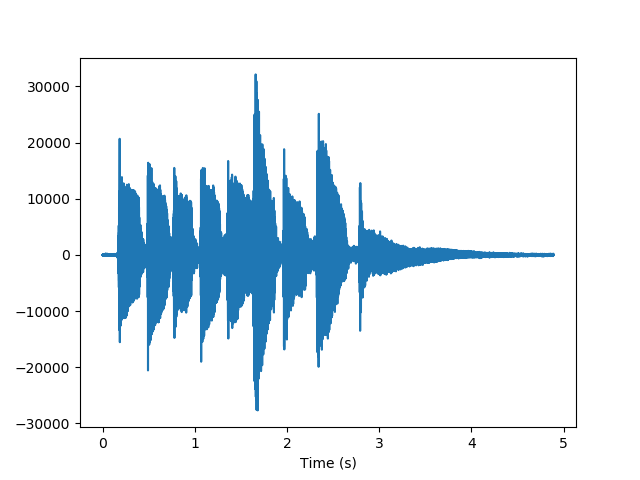
\includegraphics[width=7.5cm,height=7.0cm]{ch17/figures/audio.png}
    \caption{Audio signal}
    \label{audio_plot}
\end{marginfigure}
The length in seconds can be computed as $\text{time in seconds}=(\text{number of samples})(\text{sample spacing})$ which in this case is $t=215678/44100\approx 4.89$, so around a 5 seconds long signal. From Figure \ref{audio_plot} we see that the signal is around 5 seconds long. 

\item The following code shown in Listing \ref{code16_5} will compute and print the spectogram for the audio signal. 
\begin{lstlisting}[language=Python, caption=Spectogram code,label=code16_5]
import numpy as n
import matplotlib.pyplot as plt
import scipy.io.wavfile
import scipy.signal as ss

# function to convert to dB
def convert_to_decibel(x):
    return 10*n.log10(n.abs(x)**2)

audio = scipy.io.wavfile.read("b.wav")
sample_rate = audio[0]
# read only one channel of the stereo signal
signal = audio[1][:,0]

# function to compute the spectogram
def spectogram(signal,delta_n,N,M):
    # have a signal x of length L
    # we divide the signal into sub arrays of length N, the step size is then delta_n
    # the maximum time units are then L/delta_n

    # M - length of FFT
    # N - length of window
    # delta_n - step size in time

    # window function (Hann window)
    w = ss.hann(N)

    # length of signal
    L = len(signal)

    # compute the maximum number of time steps
    t_max = int((L-N)/delta_n)

    # allocate space for the spectogram and sub_arrays
    H = n.zeros([t_max,M],dtype=n.complex64)
    sub_array = n.zeros(N)

    # step through the signal
    for i in range(t_max):
        # get a sub_array and then fft it with the window and store it in H
        sub_array[0:N] = signal[i*delta_n + n.arange(N)]
        H[i,:] = n.fft.fft(sub_array*w,M)

    return H

M = 10480
N = 2000
delta_n = 40

# compute the spectogram
spect = spectogram(signal,delta_n,N,M)

# partition the axes correctly with units of Hertz and seconds
freqs = n.fft.fftfreq(M,d=1.0/sample_rate)
time = delta_n*n.arange(spect.shape[0])/sample_rate

# create the spectogram plot, limiting frequency to (0,1500) Hz
plt.pcolormesh(time,freqs[0:M//2],n.transpose(convert_to_decibel(spect[:,0:M//2])),vmin=40)
plt.xlabel("Time (s)")
plt.ylabel("Frequency (Hz)")
plt.ylim(0,1500)
plt.colorbar()
plt.show()
\end{lstlisting}

\item The output of Listing \ref{code16_5} is shown in Figure \ref{fur_elise_spectogram}.
\begin{figure}[h!]
    \centering
    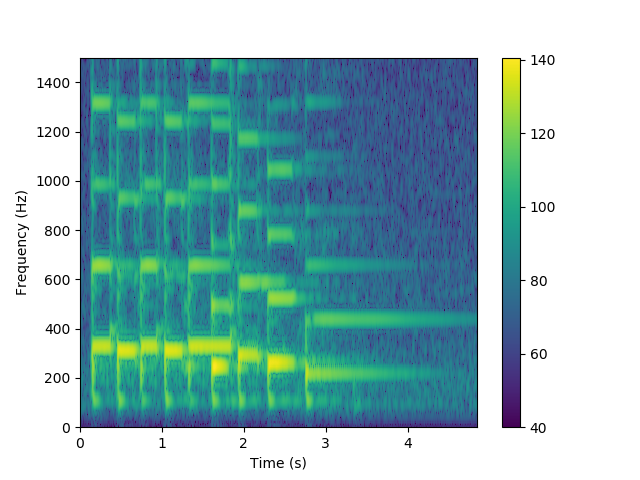
\includegraphics[scale=1.0]{ch17/figures/fur_elise_spectogram.png}
    \caption{Für Elise spectogram}
    \label{fur_elise_spectogram}
\end{figure}

\item Instruments don't produce pure frequency tones, so there will be harmonics, which can be seen in Figure \ref{fur_elise_spectogram}. Different instruments emphasize different harmonics,
giving each instrument its respective sound among other factors. 

\item Comparing the spectogram with the frequency table, one can read that the musical phrase is E D\# E D\# E B D C A. You can compare this with sheet music for the piece, which is the correct phrase. 

\end{enumerate}
\end{enumerate}